\documentclass{article}

\usepackage{float}
\usepackage{listings}
\usepackage{amsmath}
\usepackage[hidelinks]{hyperref} 	% per nascondere le box intorno alle voci dell'indice
\usepackage{graphicx}
\usepackage{subfiles}
% \usepackage[margin=1.5in]{geometry} % per diminuire il margine a bordo pagina
\usepackage[bottom]{footmisc} 		% per mettere il footnote a pie' di pagina
\usepackage[affil-it]{authblk}
\usepackage{listings}
\usepackage[T1]{fontenc}

\bibliographystyle{plain}
\usepackage{natbib}

\lstset{
  frame=bt,
  %frameround=tttt,
 %mathescape=true,
  %  language=R,
   breaklines=true,
   showstringspaces=false,
   columns=flexible,
   numbers=none,
  %  commentstyle=\color{blue},
  % stringstyle=\color{gray},
   %stringstyle=\color{purple},
  %  basicstyle=\ttfamily\footnotesize
  basicstyle=\ttfamily\footnotesize,
   %literate=*{\$}{{\textcolor{arsenic}{\$}}}{1},
   tabsize=4
 }

% \bibliographystyle{plain}
% \usepackage{natbib}

% \hypersetup{
%     colorlinks=false, %set true if you want colored links
%     linktoc=all,     %set to all if you want both sections and subsections linked
%     linkcolor=blue,  %choose some color if you want links to stand out
% }

% \setcounter{secnumdepth}{5}
% \setcounter{tocdepth}{5}

\setlength{\parindent}{0in}
\newcommand{\floor}[1]{\left\lfloor #1 \right\rfloor}
\newcommand{\ceil}[1]{\left\lceil #1 \right\rceil}

% \date{}

% \renewcommand*\contentsname{Indice}

\begin{document}

\begin{titlepage}
  % \vspace*{\stretch{1.0}}
  \begin{center}
     \Large\textsc{Machine Learning course\\University of Parma - A.Y. 2020/2021}\\
     \vspace{1cm}
     \Large\textbf{An introduction to the Caret package}\\
     \vspace{1cm}
     
      \large{\textsc{Author}: \texttt{Francesco Vetere}\\ \small \textsc{e-mail:} \href{mailto:francesco.vetere@studenti.unipr.it}{\texttt{francesco.vetere@studenti.unipr.it}} }
  \end{center}
  \vspace*{\stretch{2.0}}
\end{titlepage}

\tableofcontents

\pagebreak

\section{Introduction}
Caret (short for \textbf{C}lassification \textbf{A}nd \textbf{RE}gression \textbf{T}raining) is a comprehensive framework for building machine learning models in R.\\

\textbf{R} is a language and environment for statistical computing and graphics, widely used in AI and ML applications.\\
It is open-source, provides many statistical techniques (such as tests, classification, clustering, etc.), and has many packages that can be used to solve different problems.\\

Sometimes the syntax and the way to implement ML algorithms differ across packages: \textbf{Caret} is an R package that provides a uniform interface to the various existing modeling functions.\\
In particular, it offers tools for data splitting, data pre-processing, model creation and tuning, and many more.\\

The aim of this paper is to introduce the developer to the Caret package: starting from the installation process, it will be then shown how to use Caret to build machine learning models.\\
Finally, some practical examples of Multi-Layer Perceptrons will be presented.\\

\pagebreak

\section{Installation and prerequisites}
\subsection{R}
R is a multi-platform environment, available for various OS.\\
In this paper, the installation process will be shown for Ubuntu 20.04 LTS\\
(however, it is very similar for other Linux distros).\\

Precompiled binaries of R are available for various OS on \textbf{CRAN} \href{https://cloud.r-project.org/}{\texttt{(https://cloud.r-project.org/)}}, a network of ftp and web servers around the world that stores identical, up-to-date, versions of code and documentation for R.\\

However, with Ubuntu it is also possible to install it directly from terminal with \texttt{sudo}, or as a root user:\\

\begin{lstlisting}
  # update indices
  apt update -qq

  # install two helper packages we need
  apt install --no-install-recommends software-properties-common dirmngr

  # import the signing key (by Michael Rutter) for these repo
  apt-key adv --keyserver keyserver.ubuntu.com --recv-keys E298A3A825C0D65DFD57CBB651716619E084DAB9

  # add the R 4.0 repo from CRAN -- adjust 'focal' to 'groovy' or 'bionic' as needed
  add-apt-repository "deb https://cloud.r-project.org/bin/linux/ubuntu $(lsb_release -cs)-cran40/"

  # install R and its dependencies
  apt install --no-install-recommends r-base

\end{lstlisting}

\vspace{3mm}
Now, R and its dependecies are installed: typing the command \texttt{R} in the terminal will launch the R interpreter.\\

\subsection{RStudio}
In order to write R code, a very popular IDE is \textbf{RStudio}, available for many platforms \href{https://www.rstudio.com/products/rstudio/download/}{\texttt{(https://www.rstudio.com/products/rstudio/download/)}}.
\\

Once the correct version of the software has been chosen, a \texttt{.deb} package will be downloaded: it is useful to install it with \texttt{gdebi}, a command that will ensure that all additional prerequisites for RStudio are fullfilled (such as \texttt{clang} and others).\\

\begin{lstlisting}
  # install RStudio and its dependencies
  gdebi rstudio-1.4.1717-amd64.deb
\end{lstlisting}

\pagebreak

\subsection{Caret}
In order to install the Caret package, it's sufficient to open RStudio (or directly the R interpeter) and execute the following line of code:\\

\begin{lstlisting}
  install.packages('caret', dependencies = TRUE)
\end{lstlisting}

Caret will be downloaded from CRAN, together with its dependencies.\\

Once the process is ended, Caret is ready to be included in a normal R program with the following directive:\\

\begin{lstlisting}
  library('caret')
\end{lstlisting}

\pagebreak

\section{Core elements of Caret}
\subsection{Data preprocessing}
\subsubsection{createDataPartition()}
Once a dataset has been loaded with standard R functions (i.e.: \texttt{read.csv()}), the first step is to split it into a training set and a test set.\\
(Note: when we talk about test set, in this circumstance, we are always referring to it as a validation set).\\

In order to do this, Caret offers a handy \texttt{createDataPartition} function.\\

\textbf{Syntax}
\begin{verbatim}
  createDataPartition(
    y,
    times = 1,
    p = 0.5,
    list = TRUE
  )

\end{verbatim}

\textbf{Arguments}\\

\texttt{y}: a vector of outcomes, useful because it allows Caret to preserve\\
\phantom{....}the proportion of the categories specified in this parameter.\\
\texttt{times}: the number of partitions to create.\\
\texttt{p}: the percentage of data that goes to training.\\
\texttt{list}: TRUE if the results should be in a list;\\
\phantom{.........} FALSE if the results should be in a matrix of dimensions\\
\phantom{.........} \texttt{[floor(p * length(y)), times]}\\

\textbf{Return value}\\

A list or matrix of row position integers corresponding to the training data.\\

\pagebreak

\textbf{Example}\\
\begin{lstlisting}
# Load the caret package
library(caret)

# Import dataset
dataset <- read.csv('../datasets/iris-dataset.csv')

# Create the training and test datasets
set.seed(100)

# Step 1: Get row numbers for the training data
trainRowNumbers <- createDataPartition(dataset$Species, p=0.8, list=FALSE)

# Step 2: Create the training dataset
trainData <- dataset[trainRowNumbers,]

# Step 3: Create the test dataset
testData <- dataset[-trainRowNumbers,]

print(nrow(dataset))      # 150
print(nrow(trainData))    # 120
print(nrow(testData))     # 30
\end{lstlisting}

\subsubsection{preProcess()}
Often some kind of preprocessing over our dataset can be useful, like normalization or standardization.\\
Caret make this process easy, providing the \texttt{preProcess} function.\\

\textbf{Syntax}
\begin{verbatim}
  preProcess(
    x,
    method = c("center", "scale")
    ...
  )
\end{verbatim}

\textbf{Arguments}\\

\texttt{x}: a matrix or data frame.\\
\texttt{method}: a character vector specifying the type of processing. \\
\phantom{..............} Possible values are:\\
\phantom{..............} "range": Normalize values so it ranges between 0 and 1\\
\phantom{..............} "center": Subtract Mean\\
\phantom{..............} "scale": Divide by standard deviation\\
\phantom{..............} and many more...\\
...\\

\textbf{Return value}\\

A list of various statistics, which will be transormed in the desired data frame calling the \texttt{predict} function, as shown in the example below.\\

\textbf{Example}\\
\begin{lstlisting}
print("before\n")
print(head(dataset))

# We want to normalize our dataset
preProcess_range_model <- preProcess(dataset, method='range')
dataset <- predict(preProcess_range_model, newdata = dataset)

print("after\n")
print(head(dataset))
\end{lstlisting}

\pagebreak

\subsection{Model training and tuning}
\subsubsection{train()}
Once data are ready, the next step is to build the machine learning model, choosing its hyperparameters and its training control strategies.\\

Caret provides a huge list of possible models, currently 238.\\
See \href{https://topepo.github.io/caret/available-models.html}{\texttt{https://topepo.github.io/caret/available-models.html}} for further details.\\

Each model may be implemented using a different backend library, but Caret's interface remains the same, simplifying the developer's work.\\

In particular, Caret provides a \texttt{train} function that performs all the necessary work in order to train and tune a specific model, that can be used transparently both for regression and classification tasks.\\ 

\textbf{Syntax}
\begin{verbatim}
  train(form,
        data,
        method='rf',
        trControl=trainControl(),
        tuneGrid=NULL,
        ...
       )
\end{verbatim}

\pagebreak

\textbf{Arguments}\\

\texttt{form}: A formula of the form \texttt{y $\sim$  x1 + x2 + ...} for dividing outcome from \phantom{..........}
predictors.\\
\texttt{data}: Data frame from which variables specified in \texttt{form} are taken.\\
\texttt{method}: A string specifying which classification or regression model to use.\\
\phantom{..............}Possible values are found using \texttt{names(getModelInfo())}\\
\texttt{trControl}: A function defining the training control strategy.\\
\texttt{tuneGrid}: A data frame that specifies the tuning values for the chosen \texttt{method}.\\
...\\

\textbf{Return value}\\

A list which describes the model.\\

\textbf{Example}\\
\begin{lstlisting}
# Train using a neural network (SLP) with 3 neurons, no weight decay,
# and K-fold cross-validation (K=10) as training control
model <- train(form=Species ~ .,       # outcome ~ predictors
                data=trainData,
                method='nnet',
                trControl=trainControl(method="repeatedcv",number=10,repeats=10),
                tuneGrid=expand.grid(size=3,decay=0),
                trace=FALSE)           # avoids verbose output 
\end{lstlisting}

\pagebreak

\subsection{Predictions and evaluations}

\subsubsection{predict()}
When the model has been created, trained and tuned, we can start predict new outcomes from test data.\\
This is done by \texttt{predict} function.\\

\textbf{Syntax}
\begin{verbatim}
  predict(
    object,
    newdata = NULL,
    type = "raw",
    ...
  )
\end{verbatim}

\textbf{Arguments}\\

\texttt{object}: A model created with \texttt{train}.\\
\texttt{newdata}: An optional set of data to predict on.\\
\phantom{................}If NULL, then the original training data are used.\\
\texttt{type}: either "raw" or "prob", for the number/class predictions \\
\phantom{..........}or class probabilities, respectively.\\
\phantom{..........}Class probabilities are not available for all classification models.\\
...\\

\textbf{Return value}\\

A vector of predictions if \texttt{type} = "raw", or a data frame of class probabilities for \texttt{type} = "prob".\\

\textbf{Example}\\
\begin{lstlisting}
# Predict "Species" attribute for data in testData using the model trained before
prediction <- predict(model, testData[-5])
\end{lstlisting}

\pagebreak

\subsubsection{confusionMatrix()}
Once the predictions are made, it is possible to compare the predictions versus the actual data, generating also some evaluation metrics.\\
This is done by \texttt{confusionMatrix} function.\\

\textbf{Syntax}
\begin{verbatim}
  confusionMatrix(
    data,
    reference,
    mode = "sens_spec",
    ...
  )
\end{verbatim}

\textbf{Arguments}\\

\texttt{data}: A factor of predicted classes.\\
\texttt{reference}: A factor of classes to be used as the true results.\\
\texttt{mode}: A single character string either "sens\_spec", "prec\_recall",\\
\phantom{..........}or "everything"\\
...\\

\textbf{Return value}\\

A list containing the table representing the confusion matrix and the various evaluation metrics selected with \texttt{mode}.\\

\textbf{Example}\\

\begin{lstlisting}
  # Create a confusion matrix with all possible evaluation metrics
  cm <- confusionMatrix(reference = as.factor(testData$Species), 
         data = prediction, mode='everything')
  print(cm)
\end{lstlisting}

\pagebreak

Looking at the output generated, we can observe that not only a confusion matrix has been generated, but also some relevant statistics.\\

From the confusion matrix, we can observe how exactly 1 instance of Iris-virignica has been misclassified as Iris-versicolor.\\
This led to a global accuracy of 96.67\%.\\

Also, for each class some separate metrics are computed, such as sensitivity, specificity, precision, recall, etc.\\

\begin{lstlisting}
  Confusion Matrix and Statistics

                  Reference
Prediction        Iris-setosa Iris-versicolor Iris-virginica
  Iris-setosa              10               0              0
  Iris-versicolor           0               9              0
  Iris-virginica            0               1             10

Overall Statistics
                           
  Accuracy : 0.9667          
  ...            

Statistics by Class:

                      Class: Iris-setosa Class: Iris-versicolor Class: Iris-virginica
  Sensitivity                      1.0000                 0.9000                1.0000
  Specificity                      1.0000                 1.0000                0.9500
  Precision                        1.0000                 1.0000                0.9091
  Recall                           1.0000                 0.9000                1.0000
  ...
\end{lstlisting}

\pagebreak

\section{Examples}
In this final section, some complete examples of MLPs are presented.\\
Caret offers various models in order to build MLPs, such as \texttt{'nnet'}, \texttt{'mlp'}, \texttt{'mlpML'}, \texttt{'mlpKerasDropout'}, \texttt{'mlpKerasDropoutCost'} and many more.\\

Each of them provides a different set of tuning parameters that need to be assigned in the \texttt{tuneGrid} parameter of the \texttt{train} function.\\

\subsection{Classification with MLP (1 layer)}
In this first example, the objective is to perform a classification task over the well known iris dataset, using a Multi-Layer Perceptron with a single layer of 3 neurons.\\
For this task, the \texttt{nnet} model is used.\\

\lstinputlisting{"../examples/MLP-classification1.r"}

\pagebreak

This is the output generated, from which we can observe that the 30 test istances have been classified with an accuracy of 96.67\%.\\

Looking at the confusion matrix, we note that only 1 instance has been misclassified.\\

Of course, a lot of metrics have been generated because we selected \texttt{'everything'} as value for the \texttt{mode} parameter of the confusion matrix.\\

\begin{lstlisting}
 [1] Iris-setosa     Iris-setosa     Iris-setosa     Iris-setosa     Iris-setosa     Iris-setosa    
 [7] Iris-setosa     Iris-setosa     Iris-setosa     Iris-setosa     Iris-versicolor Iris-versicolor
[13] Iris-versicolor Iris-versicolor Iris-versicolor Iris-versicolor Iris-versicolor Iris-virginica 
[19] Iris-versicolor Iris-versicolor Iris-virginica  Iris-virginica  Iris-virginica  Iris-virginica 
[25] Iris-virginica  Iris-virginica  Iris-virginica  Iris-virginica  Iris-virginica  Iris-virginica 

Levels: Iris-setosa Iris-versicolor Iris-virginica

Confusion Matrix and Statistics

                 Reference
Prediction        Iris-setosa Iris-versicolor Iris-virginica
  Iris-setosa              10               0              0
  Iris-versicolor           0               9              0
  Iris-virginica            0               1             10

Overall Statistics
                                          
               Accuracy : 0.9667          
               ...            

Statistics by Class:

                     Class: Iris-setosa Class: Iris-versicolor Class: Iris-virginica
Sensitivity                      1.0000                 0.9000                1.0000
Specificity                      1.0000                 1.0000                0.9500
...

\end{lstlisting}

\pagebreak

\subsection{Classification with MLP (3 layers)}
In this example, we want to adapt the previous problem using a 3-layers MLP.\\

This can be done using the \texttt{mlpML} model, which allows to specify up to 3 layers as tuning parameters (other models like \texttt{mlpSGD} provide also more sophisticated tuning parameters, such as \texttt{learn\_rate} and \texttt{momentum}).\\

\lstinputlisting{"../examples/MLP-classification2.r"}

\pagebreak

This is the output generated, from which we can observe that we obtained an accuracy of 56.67\%.\\

This accuracy, much lower than the one we obtained with a simpler MLP, indicates that this model is not so adequate for the task: it is too complex, and thus it overfits data.\\

Moreover, not only accuracy is worse, but almost every other computed metric.\\

\begin{lstlisting}
  [1] Iris-setosa     Iris-setosa     Iris-setosa     Iris-setosa     Iris-setosa     Iris-setosa     Iris-setosa    
  [8] Iris-setosa     Iris-setosa     Iris-setosa     Iris-versicolor Iris-versicolor Iris-setosa     Iris-versicolor
 [15] Iris-versicolor Iris-setosa     Iris-setosa     Iris-versicolor Iris-versicolor Iris-versicolor Iris-versicolor
 [22] Iris-versicolor Iris-versicolor Iris-versicolor Iris-versicolor Iris-versicolor Iris-versicolor Iris-versicolor
 [29] Iris-versicolor Iris-versicolor

 Levels: Iris-setosa Iris-versicolor Iris-virginica

 Confusion Matrix and Statistics
 
                  Reference
 Prediction        Iris-setosa Iris-versicolor Iris-virginica
   Iris-setosa              10               3              0
   Iris-versicolor           0               7             10
   Iris-virginica            0               0              0
 
 Overall Statistics
                                           
                Accuracy : 0.5667          
                ... 

 Statistics by Class:
 
                      Class: Iris-setosa Class: Iris-versicolor Class: Iris-virginica
 Sensitivity                      1.0000                 0.7000                0.0000
 Specificity                      0.8500                 0.5000                1.0000
 ...
\end{lstlisting}

\pagebreak

\subsection{Regression with MLP}
In this final example, the task is to predict the value of a potential car sale (i.e. how much a particular person will spend on buying a car) for a customer on the basis of the following attributes: age, gender, average miles driven per day, personal debt, monthly income.\\

This can be done for example using a \texttt{mlp} model, specifying \texttt{RMSE} as the chosen metric.\\

\lstinputlisting{"../examples/MLP-regression.r"}

\pagebreak

This is the output generated, from which we can observe that the 192 test istances have been predicted with a final RMSE of 9296.64.\\

\begin{lstlisting}
  6           16           19           25           27           
  8.551736e+03 1.946015e+04 8.551736e+03 1.605100e+04 1.946015e+04 

  ...

  920          929          944          952          955 
  8.551736e+03 1.090841e+04 1.605100e+04 8.551736e+03 2.460274e+04 

  Multi-Layer Perceptron 
  
  963 samples
    5 predictor
  
  Pre-processing: centered (5), scaled (5) 
  Resampling: Cross-Validated (3 fold, repeated 3 times) 
  Summary of sample sizes: 642, 643, 641, 642, 642, 642, ... 
  Resampling results:
  
    RMSE      Rsquared   MAE     
    9296.637  0.2369883  7287.627
\end{lstlisting}

\pagebreak

Of course, an RMSE value is not so immediate to be interpreted, unlike an accuracy value.\\
To have a better understanding of how the model performs, we can plot the real outputs vs the predicted outputs, for every instance of the test set.\\

We can see that the model is not so precise in its predictions: in this case, it underfits its data.\\

\begin{figure}[H]
  \centering
  \hspace*{-0.8in}
  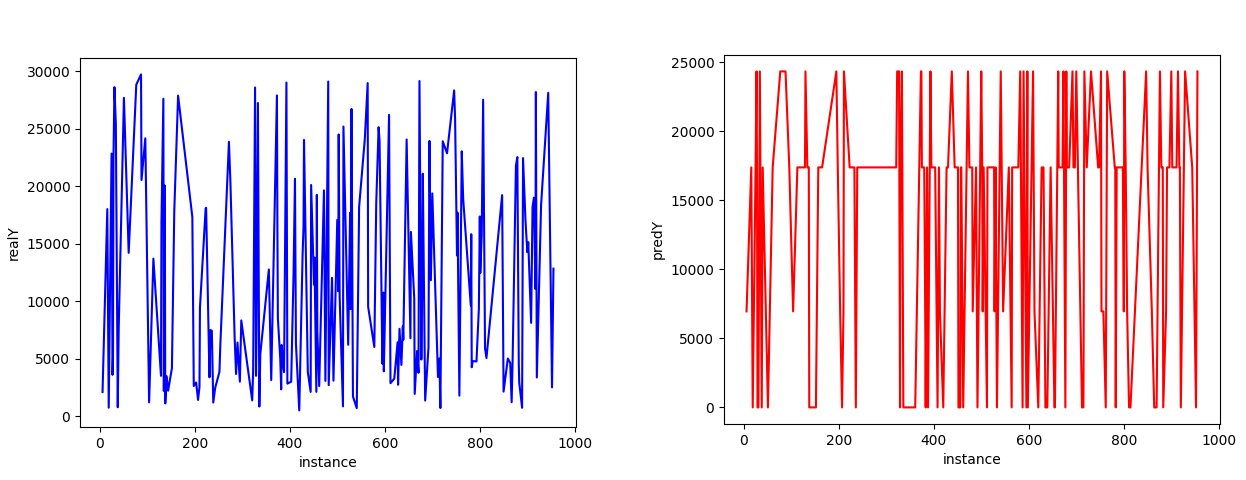
\includegraphics[scale=0.5]{realY-vs-predY.png}
  \caption{real outputs vs predicted outputs}
\end{figure}

\pagebreak

\renewcommand\refname{References}
%\addcontentsline{toc}{section}{Riferimenti bibliografici}
\subfile{bibliography.tex}
\addcontentsline{toc}{section}{References}

\end{document}